\documentclass[cs4size,a4paper,nofonts]{ctexart}
\usepackage[utf8]{inputenc}
\def\tjf{{\tt{田劲锋}}}
\def\titlec{企业应用集成系统}
\def\version{V0.0.9}
\usepackage[a4paper,margin=3cm]{geometry} % 页面设置
\usepackage[x11names]{xcolor}
\usepackage[unicode,breaklinks=true,
colorlinks=true,linkcolor=Blue4,anchorcolor=purple,citecolor=cyan,urlcolor=magenta,
pdftitle={\titlec \version},pdfauthor={\tjf}]{hyperref}

%\CTEXsetup[number=\chinese{section}, format={\large\sf\bfseries}]{section}
\usepackage{latexsym,amsmath,amssymb,bm}
\usepackage{wasysym}
\usepackage{marvosym}
\usepackage{multicol}

\setmainfont{Times New Roman}
\setCJKmainfont[BoldFont={SimHei}]{SimSun}  % 主要字体:宋体、黑体
\setCJKsansfont[BoldFont={STZhongsong}]{STFangsong} % 次要字体:仿宋、中宋
\setCJKmonofont{KFKai} % 等宽字体:楷体

\CJKsetecglue{\hspace{0.1em}}
\renewcommand\CJKglue{\hskip -0.3pt plus 0.08\baselineskip}
\frenchspacing
\widowpenalty=10000
\linespread{1.2} % 行距

\usepackage[inline]{enumitem} % 调整列表样式
\setlist{noitemsep}
\setlist[itemize]{topsep=0pt,partopsep=0pt,itemsep=0pt,parsep=0pt,labelindent=\parindent,leftmargin=*,align=right}
\setlist[enumerate]{topsep=0pt,partopsep=0pt,itemsep=0pt,parsep=0pt,labelindent=\parindent,leftmargin=*,align=right}
\setlist[enumerate,1]{label={\arabic{section}.\arabic{subsection}.\arabic*}}
\setlist[enumerate,2]{label*={.\arabic*}}

%\makeindex
\pagestyle{plain}

\begin{document}

%%%% 开始 %%%%

\title{\bf\titlec~\version\footnote{本文档托管在 GitHub 上,PDF 文件:\url{https://github.com/kingfree/haut/raw/master/se/eai.pdf},\TeX 源文件:\url{https://github.com/kingfree/haut/blob/master/se/eai.tex}。}}
\author{软件工程1305班~\quad\tjf\quad~201316920311}
\maketitle

\begin{multicols}{2}
\tableofcontents
\end{multicols}

\section{需求分析}
\subsection{业务需求}

企业应用集成(Enterprise Application Integration, EAI)是一个或多个系统的集合,并使两个以上的后台应用能够作特定数据的统一管理系统,并能保证这些后台应用同步良好。这样的系统可以为单个公司提供其所有信息的集中访问点。

通过应用集成,提高业务流程的自动化程度,获得如下好处:

\begin{itemize}
\item 增强业务处理的可靠性
\item 缩短处理时间
\item 减少人工干涉
\item 保证数据一致性
\item 获得更高质量的报表数据
\item 降低运营成本
\end{itemize}

本系统将来进行可以通过插件方式进行扩展,组合成功能全面的企业资源计划(Enterprise Resource Planning, ERP)系统。

\subsection{用户需求}

对于小型中型的商业公司,通常会使用多个软件系统来处理不同的事务。用户手工操作资金结算系统、发票管理系统、销售管理系统、客户服务系统,其数据都是手工完成输入的,工作时要打开多个软件,在不同的窗口之间复制、粘贴,甚至使用电子表格来处理软件系统没有提供的功能。

用户需要一个集成平台系统,尽可能来整合这些软件系统,从而减轻工作量,减少错误发生。

系统需要支持这些功能:

\begin{itemize}
\item 追踪单个请求处理状态
\item 保存用户请求日志
\item 生成各种审计报告
\item 保存系统响应日志
\item 以同步或异步的方式处理请求
\item 回滚处理流程机制
\item 搜索条目和内容
\item 事务中断处理
\end{itemize}

由于并没有具体的底层平台,该系统应开发成一个可扩展的框架(Framework),提供具体的应用程序接口(Application Programming Interface, API)而不限于图形用户界面(Graphical User Interface, GUI)。

%假设现有的系统有:

%\paragraph{结算系统}

%\paragraph{销售管理系统}

%\paragraph{客户服务系统}

% \subsection{系统需求}

\subsection{功能需求}

\begin{enumerate}
\item 【平台通用】
系统处理来自各方的请求,该机制不会限制用户或其他系统,也不限制开发环境、编程语言和操作系统。
\item 【调用接口】
系统提供一个不依赖于环境的交互接口,使用机器和人皆可读的 XML 格式可以提供一个这样的中间平台。
\item 【日志记录】
要求详细记录经过系统产生的一切处理过程,包括但不限于这些信息:编号、处理情况、提交和解决时间、处理方案和步骤。
\item 【日志查询】
提供查询记录日志的功能,用户可以按关键字查询、排序以及按条件查询。
\item 【用户验证】
提供用户注册和登录功能,为每个用户产生其需要的数据和界面。
\item 【用户权限】
为不同的用户分配不同的权限和角色,保障系统安全性和业务稳定性。用户权限设置要灵活,然而根用户例外。
\item 【用户锁定】
对于多次执行了非法操作的用户,如多次输错密码,系统将自动锁定用户一定时间,并有管理员决策是否解除锁定。
\item 【集成扩展】
系统要可以实现新增功能和业务流程的插入和修改功能,实现集成系统的扩展,以便适应用户不断变化的业务需求。
\item 【业务组合】
系统将多项任务组合成单个逻辑的用户请求,通过把若干相关的处理过程整合成为一个请求,用户可以将一系列相关操作组合成逻辑上的统一整体,并包含在单个请求中进行处理。
\item 【输入验证】
系统要验证数据输入的合法性,这是保证系统能够正常运行的必要条件。通过操作进行之前的输入验证和修正,可以预防后期修正导致的一连串棘手问题。
\item 【业务处理】
需要在请求处理过程中落实业务规则,验证用户通用的要求和自定义要求,根据不同情况处理状态和数据库,在此基础上制作数据报表和性能报表。
\item 【请求回滚】
对于包含多个步骤的处理请求,有些可以容忍的错误可以记录在日志中,有些错误不可容忍,需要中止整个请求的处理,甚至需要恢复请求之前的数据系统状态。
\item 【管理报告】
日志查询的升级版,提供图表形式的日志数据。通过对日志数据的分析,系统生成不同种类的报告提供给系统管理员分析和检查问题。
\item 【实时警报】
对于严重的系统错误,影响到了用户利益,应当提供途径向相关人员发送警报信息,以便进一步处理。方式包括但不限于电子邮件、手机短信、即时通讯等。
\item 【灾难恢复】
当系统运转过程中产生了不可避免的意外事故,如断电等,将导致处理结果不完整。有必要在分解请求的基础上,及时保存请求处理到数据库中,同时提供措施以便恢复用户提交而未能及时处理的任务。

\end{enumerate}

\section{需求建模}

\subsection{数据流图}

图~\ref{dfd0}~描述了系统最顶层的数据流。Web 服务器从用户处接收业务处理请求的消息,服务器接收到请求,将请求历史记录入日志,并将请求的业务转发给后台 EAI 系统,再由 EAI 系统来处理业务并返回业务处理情况。

\begin{figure}[htp]
\centering
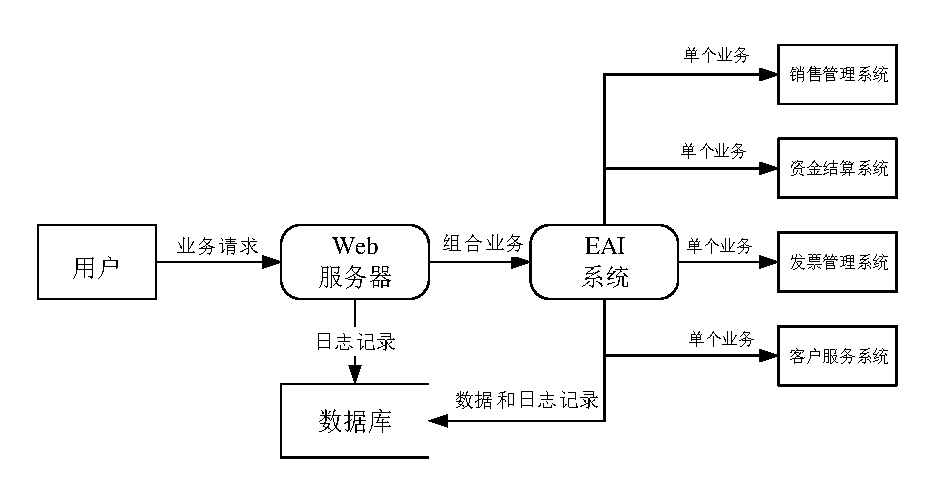
\includegraphics[width=\textwidth,page=1]{images/dfd.pdf}
\caption{\label{dfd0}系统顶级数据流图}
\end{figure}

顶级数据流包含两个主要的处理逻辑,这里将其描述为一级数据流图:

图~\ref{dfd1.1}~描述了用户请求的数据流程,也就是 Web 服务器的处理流程。用户发起一个业务请求(在 Web 中表现为GET 或 POST请求),服务器接收调用消息,验证用户身份保证会话有效性,记录日志,将消息调用转发给 EAI 后台并接收后台返回的信息显示给用户。

\begin{figure}[htp]
\centering
\includegraphics[width=\textwidth,page=2]{images/dfd.pdf}
\caption{\label{dfd1.1}一级数据流图:用户请求的处理}
\end{figure}

图~\ref{dfd1.2}~描述了 EAI 系统的后端处理的数据流程。系统接收消息调用,调用请求处理控制类生成请求对象,对请求区分同步、异步调用。对于每个业务进行分解,把分解业务交给外部系统执行,记录数据库。执行结束后更新业务状态,将响应消息返回给服务器。

\begin{figure}[htp]
\centering
\includegraphics[width=\textwidth,page=3]{images/dfd.pdf}
\caption{\label{dfd1.2}一级数据流图:EAI 系统的后端处理}
\end{figure}

% \section{用例模型}

\subsection{用例图}

图~\ref{uc1}~是该系统的用例图,用户只有两个基本用例,登录和业务请求。注意这里我们将业务请求合并为了一个用例,因为实际上我们是可以用一个类来处理这项业务的。

\begin{figure}[htp]
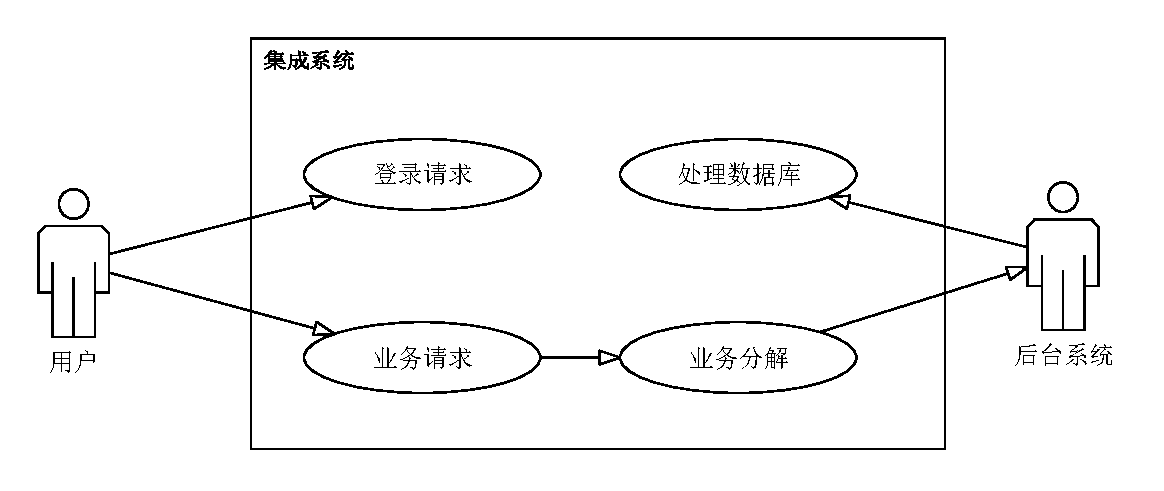
\includegraphics[width=\textwidth,page=1]{images/ucs.pdf}
\caption{\label{uc1}系统用例图}
\end{figure}

\subsection{用例描述}

\newcounter{uccounter}[subsection]
\renewcommand{\theuccounter}{\arabic{section}.\arabic{subsection}.\arabic{uccounter}}
\newcommand*{\ucref}[1]{\hyperref[{uc:#1}]{用例~\ref*{uc:#1}:#1}}
\newcommand{\usecasedes}[9]{\CTEXnoindent
%\begin{minipage}{\textwidth}
\refstepcounter{uccounter}
{{\label{uc:#1}\addcontentsline{toc}{subsubsection}{用例~\theuccounter :#1}}\bf{用例~\theuccounter :#1}}
\begin{enumerate}[label={\arabic*.}]
\item 目标

#2
\item 事件流
\begin{enumerate}[label*={\arabic*}]
\item 基本流程

#3
\begin{enumerate}[label={(\arabic*)}]
#4
\end{enumerate}
\item 可选流程

#5
\begin{enumerate}[label={(\arabic*)}]
#6
\end{enumerate}
\end{enumerate}
\item 特殊需求

#7
\item 前提条件

#8
\item 后置条件

#9
\end{enumerate}
%\end{minipage}
\CTEXindent}

\newcommand{\button}[1]{~\fcolorbox{gray}{white}{\color{black}\bf{#1}}~按钮}
\newcommand{\checkbox}[1]{~\CheckedBox{\tt{#1}}~复选框}
\newcommand{\textfield}[1]{\underline{\color{darkgray}\tt{#1}}}

\usecasedes{用户无状态登录} % #1 用例
{该用例允许用户登录,验证用户身份,并将用户状态保存在会话中。} % #2 目标
{当用户进入该系统登录页面,该用例开始执行。} % #3 基本流程
{
\item 用户输入\textfield{用户名}和\textfield{密码},按下\button{登录};
\item 系统将\textfield{密码}加密后,检查\textfield{用户名}存在且加密密码一致;
\item 生成新的会话编号并将其和当前时间记入数据库;
\item 返回并设置会话表示登录成功。
} % #4 基本流程列表
{} % #5 可选流程
{
\item 用户不存在\par
在主流程中,如果系统中没有与输入用户名匹配的用户,返回错误消息,用例结束。
\item 密码错误\par
在主流程中,加密后的密码与对应系统中用户的加密密码不一致,返回错误消息,用例结束。
} % #6 可选流程列表
{在输入过程中,用户选择了\checkbox{下次自动登录},系统需要在登录验证成功后,将会话写入状态。} % #7 特殊需求
{用户没有登录,且没有登录状态。} % #8 前提条件
{用户通过登录验证,其状态保存在会话中。} % #9 后置条件

\usecasedes{用户带状态登录} % #1 用例
{该用例允许用户不输入用户名和密码直接登陆系统。} % #2 目标
{当用户启动该系统,进入该系统任意页面,该用例开始执行。} % #3 基本流程
{
\item 检查用户是否有状态信息;
\item 检查用户状态,在数据库中找到对应的会话编号;
\item 返回并设置会话表示登录成功。
} % #4 基本流程列表
{} % #5 可选流程
{
\item 没有状态\par
用户没有状态信息,跳转到\ucref{用户无状态登录},本用例结束。
\item 无此会话\par
没有在数据库中找到对应的会话编号,返回错误消息,用例结束。
} % #6 可选流程列表
{无。} % #7 特殊需求
{用户进入该页面时已经带有状态。} % #8 前提条件
{用户通过登录验证,其状态保存在会话中。} % #9 后置条件

\usecasedes{业务请求} % #1 用例
{用户提交一个业务请求,系统分解处理该请求并返回给用户。} % #2 目标
{当用户进入指定页面填写业务表单后提交了该请求时,该用例开始执行。} % #3 基本流程
{
\item 将用户的表单内容转换成中间格式 XML;
\item 系统解析 XML 语义生成请求对象;
\item 系统确定该业务是同步处理业务还是异步处理业务;
\item 将异步请求对象加入处理队列,为同步业务新建处理对象;
\item 系统处理该对象,调用\ucref{同步业务请求}或\ucref{异步业务请求};
\item 根据处理结果,返回响应对象。
} % #4 基本流程列表
{} % #5 可选流程
{
\item 解析错误\par
用户的输入存在错误,无法正确解析成 XML,返回出错消息,用例结束。
} % #6 可选流程列表
{无。} % #7 特殊需求
{用户已登录且拥有处理该业务的权限。} % #8 前提条件
{业务处理并返回状态,记录日志。} % #9 后置条件

\usecasedes{记录日志} % #1 用例
{对于用户操作和系统的处理等动作进行记录。} % #2 目标
{系统产生一个动作时进入该用例。} % #3 基本流程
{
\item 系统获得当前动作的标记信息;
\item 系统区分该动作的日志级别;
\item 产生唯一日志编号,根据级别写入日志到数据库;
\item 系统读取并解析输出日志的参数;
\item 向指定位置输出日志消息和时间。
} % #4 基本流程列表
{} % #5 可选流程
{
\item 日志不可写\par
日志配置中指定的位置不可写入,产生警告并写入默认日志位置。
} % #6 可选流程列表
{无。} % #7 特殊需求
{无。} % #8 前提条件
{日志写出成功,转入正常业务流程。} % #9 后置条件

\usecasedes{同步业务请求} % #1 用例
{以同步的方式处理业务请求。} % #2 目标
{} % #3 基本流程
{
\item 检查预处理业务规则;
\item 解析出调用请求;
\item 调用对应的请求处理对象;
\item 检查请求类型的业务规则;
\item 请求处理对象执行必要的处理步骤;
\item 处理步骤记录必要的日志信息;
\item 处理业务后规则;
\item 生成并返回响应对象。
} % #4 基本流程列表
{} % #5 可选流程
{
\item 处理步骤出错\par
处理请求处理对象时出现错误,在系统允许的情况下结束该业务,记录业务状态;需要回滚的业务要调用回滚处理用例。
} % #6 可选流程列表
{无。} % #7 特殊需求
{系统接收到同步业务处理请求。} % #8 前提条件
{同步业务请求处理完成。} % #9 后置条件

\usecasedes{异步业务请求} % #1 用例
{以异步的方式处理业务请求。} % #2 目标
{} % #3 基本流程
{
\item 将调用请求压入消息队列;
\item 记录必要的日志信息;
\item 生成并返回响应对象。
} % #4 基本流程列表
{} % #5 可选流程
{
\item 无。
} % #6 可选流程列表
{无。} % #7 特殊需求
{系统接收到异步业务处理请求。} % #8 前提条件
{异步业务请求成功加入队列。} % #9 后置条件

\usecasedes{加入消息队列} % #1 用例
{将异步处理业务请求加入消息队列} % #2 目标
{} % #3 基本流程
{
\item 将用户请求打包为格式消息;
\item 将消息加入队列,消息队列接收消息并存储下来。
} % #4 基本流程列表
{} % #5 可选流程
{
\item 无。
} % #6 可选流程列表
{无。} % #7 特殊需求
{异步业务已解析成为处理对象。} % #8 前提条件
{业务加入消息队列,等待处理。} % #9 后置条件

\usecasedes{监控消息队列} % #1 用例
{监控程序监控消息队列并按顺序处理其中的请求对象。} % #2 目标
{} % #3 基本流程
{
\item 按照先进先出(First In First Out, FIFO)的顺序从队列中读取一个消息;
\item 处理消息;
\item 报告处理情况,记录日志和数据库。
} % #4 基本流程列表
{} % #5 可选流程
{
\item 队列为空\par
消息队列中没有消息请求,说明当前没有要处理的异步请求,用例结束。
} % #6 可选流程列表
{无。} % #7 特殊需求
{消息队列已启动} % #8 前提条件
{继续处理下一个消息。} % #9 后置条件

\usecasedes{新增请求类型} % #1 用例
{提供一个添加新的业务流程的通用接口。} % #2 目标
{} % #3 基本流程
{
\item 确定请求消息中的请求名称;
\item 通过继承公共请求类来新建处理类:
\begin{enumerate}
\item 为新的请求处理类新建一个类,声明其父类;
\item 重写处理方法;
\item 重写内部处理方法;
\item 重写回滚方法;
\item 编译测试新的处理类。
\end{enumerate}
\item 在数据库中插入相应记录,标记此类可用。
} % #4 基本流程列表
{} % #5 可选流程
{
\item 新建类名冲突\par
用户要求新建的类名与已有类名冲突,系统提示更改名称以消除冲突;
\item 类编译测试失败\par
新建类编译测试失败,标记此类不可用,直至调试成功。
} % #6 可选流程列表
{提供调试功能。} % #7 特殊需求
{系统已提供公共处理类。} % #8 前提条件
{请求类建立完成并可用。} % #9 后置条件

\usecasedes{建立业务步骤} % #1 用例
{定义一个业务并分解成为外部系统可执行的子业务。} % #2 目标
{} % #3 基本流程
{
\item 用户要求建立一个新的业务;
\item 设置请求定义信息;
\item 设置步骤定义信息;
\item 设置处理步骤与调用请求的对应关系以及各步骤的执行顺序;
\item 为请求编写请求处理类;
\item 为每个步骤编写处理步骤类;
\item 测试调用请求。
} % #4 基本流程列表
{} % #5 可选流程
{
\item 同\ucref{新增请求类型}。
} % #6 可选流程列表
{同\ucref{新增请求类型}。} % #7 特殊需求
{已有创建业务步骤的工厂类。} % #8 前提条件
{业务被分解成为可执行的子任务。} % #9 后置条件

\usecasedes{业务规则校验} % #1 用例
{校验业务是否符合预定的规则。该用例既适用于预处理校验,也适用于后处理校验。} % #2 目标
{当一个业务消息传入,系统应当检查业务规则的合法性,用例开始执行。} % #3 基本流程
{
\item 检查标签的存在性;
\item 根据条件判定的存在性;
\item 验证标签取值;
\item 自定义的其他核准操作。
} % #4 基本流程列表
{} % #5 可选流程
{
\item 验证错误\par
验证中发生严重错误,提示并记录,用例结束。
\item 验证警告\par
验证中发现错误但并不严重,以默认值代替,提示并记录。
} % #6 可选流程列表
{无。} % #7 特殊需求
{消息处理之前和消息处理之后。} % #8 前提条件
{预处理校验或后处理校验完成。} % #9 后置条件

% \usecasedes{} % #1 用例
% {} % #2 目标
% {} % #3 基本流程
% {
% \item ttt
% } % #4 基本流程列表
% {} % #5 可选流程
% {
% \item sss
% } % #6 可选流程列表
% {} % #7 特殊需求
% {} % #8 前提条件
% {} % #9 后置条件

\end{document}
